% ----------研究四
\chapter{研究四:AI生成个性化广告的心理机制探究:信息源的影响}
研究一至研究三系统地探讨了 AI 生成个性化广告的可行性及其说服效果。研究不仅验证了 AI 生成个性化广告在不同场景中的有效性,还通过文本分析和预测模型 揭示了广告内容的个性化语言特征及其对受众偏好的影响。然而,尽管 AI 生成的个性化广告在实验中表现出一定的说服力,其心理机制仍然尚未得到深入探讨。

现有个性化广告的心理机制研究主要关注信息处理方式、消费者态度和感知特征 如何影响广告的个性化效果 \citep{li2016does,dijkstra2012personalization}。然而,信息来源(source)作为影响个性化广告接受度的关键因素,尚未受到充分关注。在传统广告传播研究中,信息来源的可信度、权威性和专业性 被认为会直接影响受众对广告的态度、信息加工方式及最终的说服效果 \citep{pornpitakpan2004persuasiveness,harvey1972effect}。此外,相较于 AI 作为传播者,人类传播者往往被认为更具可信度,并对受众态度产生更大的影响 \citep{dai2024ai}。然而,在个性化广告的背景下,AI 作为广告生成者是否会影响受众对广告的信任度、真实性判断和个性化感知,目前仍缺乏系统性的研究。

信息来源对于广告传播的影响尤为关键,尤其在 AI 逐渐介入内容创作的时代,受众可能会对广告的来源做出特定假设,并基于这一假设调整其对广告的评价。因此,本研究系统地探讨信息来源对个性化广告说服效果的影响。具体而言,本研究包括两个实验:实验 1 旨在探讨个体对个性化广告生成者的感知,即当受众接触到个性化广告时,他们如何推测其信息来源(AI vs. 人类专家),以及广告内容特征是否会影响这种推测;实验 2 进一步考察在信息来源已知的情况下,AI 作为广告生成者是否会影响个性化广告的说服效果,包括受众对广告的可信度、个性化感知和态度的变化。通过这一研究框架,我们希望揭示 AI 作为个性化广告信息源的作用机制,并为 AI 生成广告在实际应用中的优化策略提供理论依据。

\section{实验1:个性化广告生成者感知}
在人工智能逐步渗透内容创作的背景下,受众如何感知AI生成的信息,尤其是个性化广告,仍然是一个尚未充分探索的重要议题。尽管AI生成文本在某些特征上可能与人类文本存在差异,但受众是否能够准确区分AI生成的内容,以及他们对AI作为信息源的感知如何影响个性化广告的接受度,仍值得进一步研究。\citet{bai2023artificial}的研究表明,相较于人类撰写的文本,AI 生成的信息通常被认为更客观、更理性,但较缺乏独特性和叙事性。然而,在信息源不明确的情况下,人们在阅读 AI 生成的信息时,往往不会直接意识到其来源。即使受试者所阅读的信息由AI生成,大多数参与者仍认为这些内容是由人类撰写的。在 AI 生成文本的条件下,94.4\%的参与者认为文本是人类创作的,而在人类文本条件下,该比例为94.7\%。这一发现表明,在某些文本类型下,AI 生成的信息在受众看来与人类创作的文本并无显著差异,受众也并不容易察觉信息的真实来源。

基于此,实验1旨在考察受众在阅读个性化广告时,对广告生成者(AI vs.人类专家)的感知。具体而言,我们关注以下问题:(1)参与者是否能够准确区分 AI 生成的个性化广告与人类专家创作的广告?(2)哪些文本特征可能影响受众对广告信息源的判断?通过探讨参与者的感知偏差,本实验将为后续研究信息来源对个性化广告说服效果的影响提供基础性证据。

\subsection{方法}

本实验采用 \textbf{2(信息创作者:AI/人类专家)}的被试间设计。AI条件选取当前表现最优的模型GPT-4,人类专家以心理学专业研究生作为代表。广告通过针对五种不同人格水平(外倾性、开放性、尽责性、宜人性、神经质)的高水平特质进行个性化设计,即分别为高外倾、高开放、高尽责、高宜人和高神经质的消费者设计了广告内容。每位被试被随机分配到一类信息创作者的广告条件,并从每个人格水平对应的 3 则广告中随机选择 1 则进行呈现。被试依次观看五则广告(对应五种人格水平),广告呈现顺序随机,且需对每则广告进行评价。

\subsubsection{被试}

通过见数平台发布实验,366名参与者自愿参加这项研究。28名参与者由于注意检查测试未通过被剔除,剩余\textbf{322}名有效被试(年龄范围= 18-58岁;\textit{M}=29.43岁;\textit{SD}=7.36;女性203名)。参与任务的每名参与者获得5元人民币作为报酬。其中注意力检测题为一道见数平台自带的题目:“今天天气不错,请选2”,若未选2,则被判定为注意力检测题未通过。

\subsubsection{实验材料}
针对2(信息创作者:AI/人类专家)*5(广告人格:外倾性/开放性/尽责性/宜人性/神经质)共10个条件生成广告材料。AI条件选取当前表现最优的模型GPT,人类专家以心理学专业研究生作为代表。根据前人文献选择中性的产品手机,广告描述避免具体品牌名以排除品牌的影响。提供给GPT和人类专家的指导语是相同的,包括对目标消费者特点的描述(个性化,具体的人格描述参考人格特质量表中的描述)以及广告基本特征的描述。每类信息创作者(AI/人类专家)针对每种人格水平生成3-5则广告。

\subsubsection{问卷测量}
本实验采用单项选择题评估参与者对个性化广告生成者的感知。具体而言,参与者在阅读每则广告后,回答“你认为这则广告的撰写者最可能是?”。选项包括:普通人/广告专家/人工智能。

\subsubsection{文本分析}
为进一步探讨广告文本的哪些特征可能影响受试者对其来源的推测,本研究采用 LIWC(Linguistic Inquiry and Word Count) 进行文本分析(详细介绍见\ref{LIWC})。鉴于本实验的核心关注点是广告来源的归因差异,因此文本分析主要聚焦于词法和句法相关的特征,以识别可能导致受试者推测广告来源为普通人、广告专家或人工智能的语言模式。具体而言,本研究主要关注 词长(Sixltr)、助词(Particle)、分析思维(Analytic)、句子长度(Words per sentence) 等句法结构特征,以及 代词使用(Pronoun)、功能词(Function words)、标点符号(Punctuation) 等可能影响文本可读性和风格的语言模式。


\subsection{结果}

为检验广告创作者(GPT-4 vs. 人类专家)是否影响受试者对广告来源的归因,本研究采用 \textbf{卡方检验)} 进行分析。结果表明(如图\ref{fig:Study4-exp1-perception}),广告创作者与参与者对广告来源的感知之间存在显著关联,$\chi^2(2) = 18.50, \textit{p} < .001$。具体而言,GPT-4 生成的广告更倾向于被归因为 AI 生成,而人类专家撰写的广告更可能被受试者认为是普通人创作的。这一发现表明,即便在广告创作者未知的情况下,参与者仍然能够在一定程度上区分AI生成和人类创作的广告,反映出 AI 生成广告在语言特征或表达方式上的潜在区别。

\begin{figure}[H]
    \centering
    \subfloat[GPT 创作者]{
        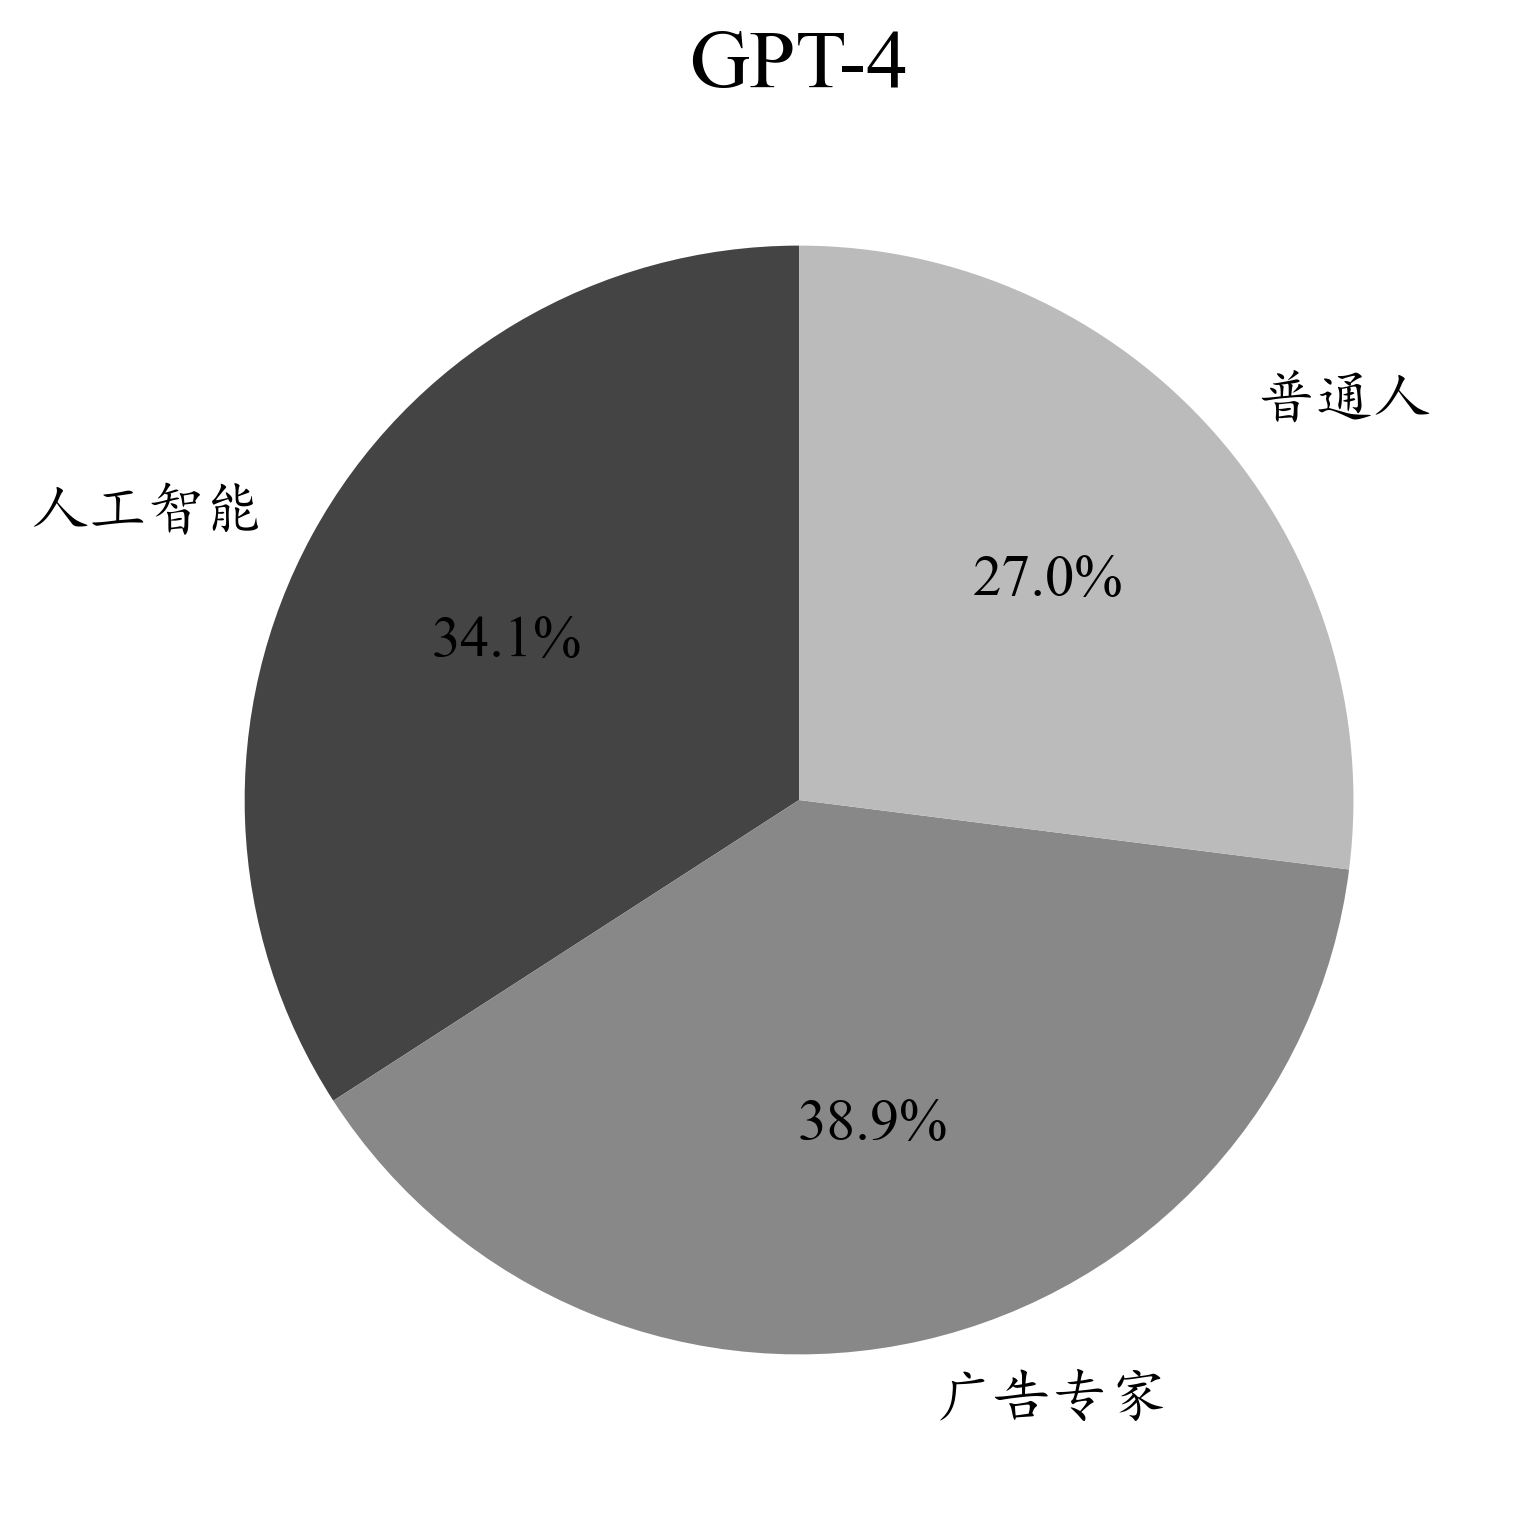
\includegraphics[width=0.4\linewidth]{Image/Study4-exp1-GPT创作者.png}
    }\hspace{2em} % 控制两张图片之间的水平间距
    \subfloat[人类专家创作者]{
        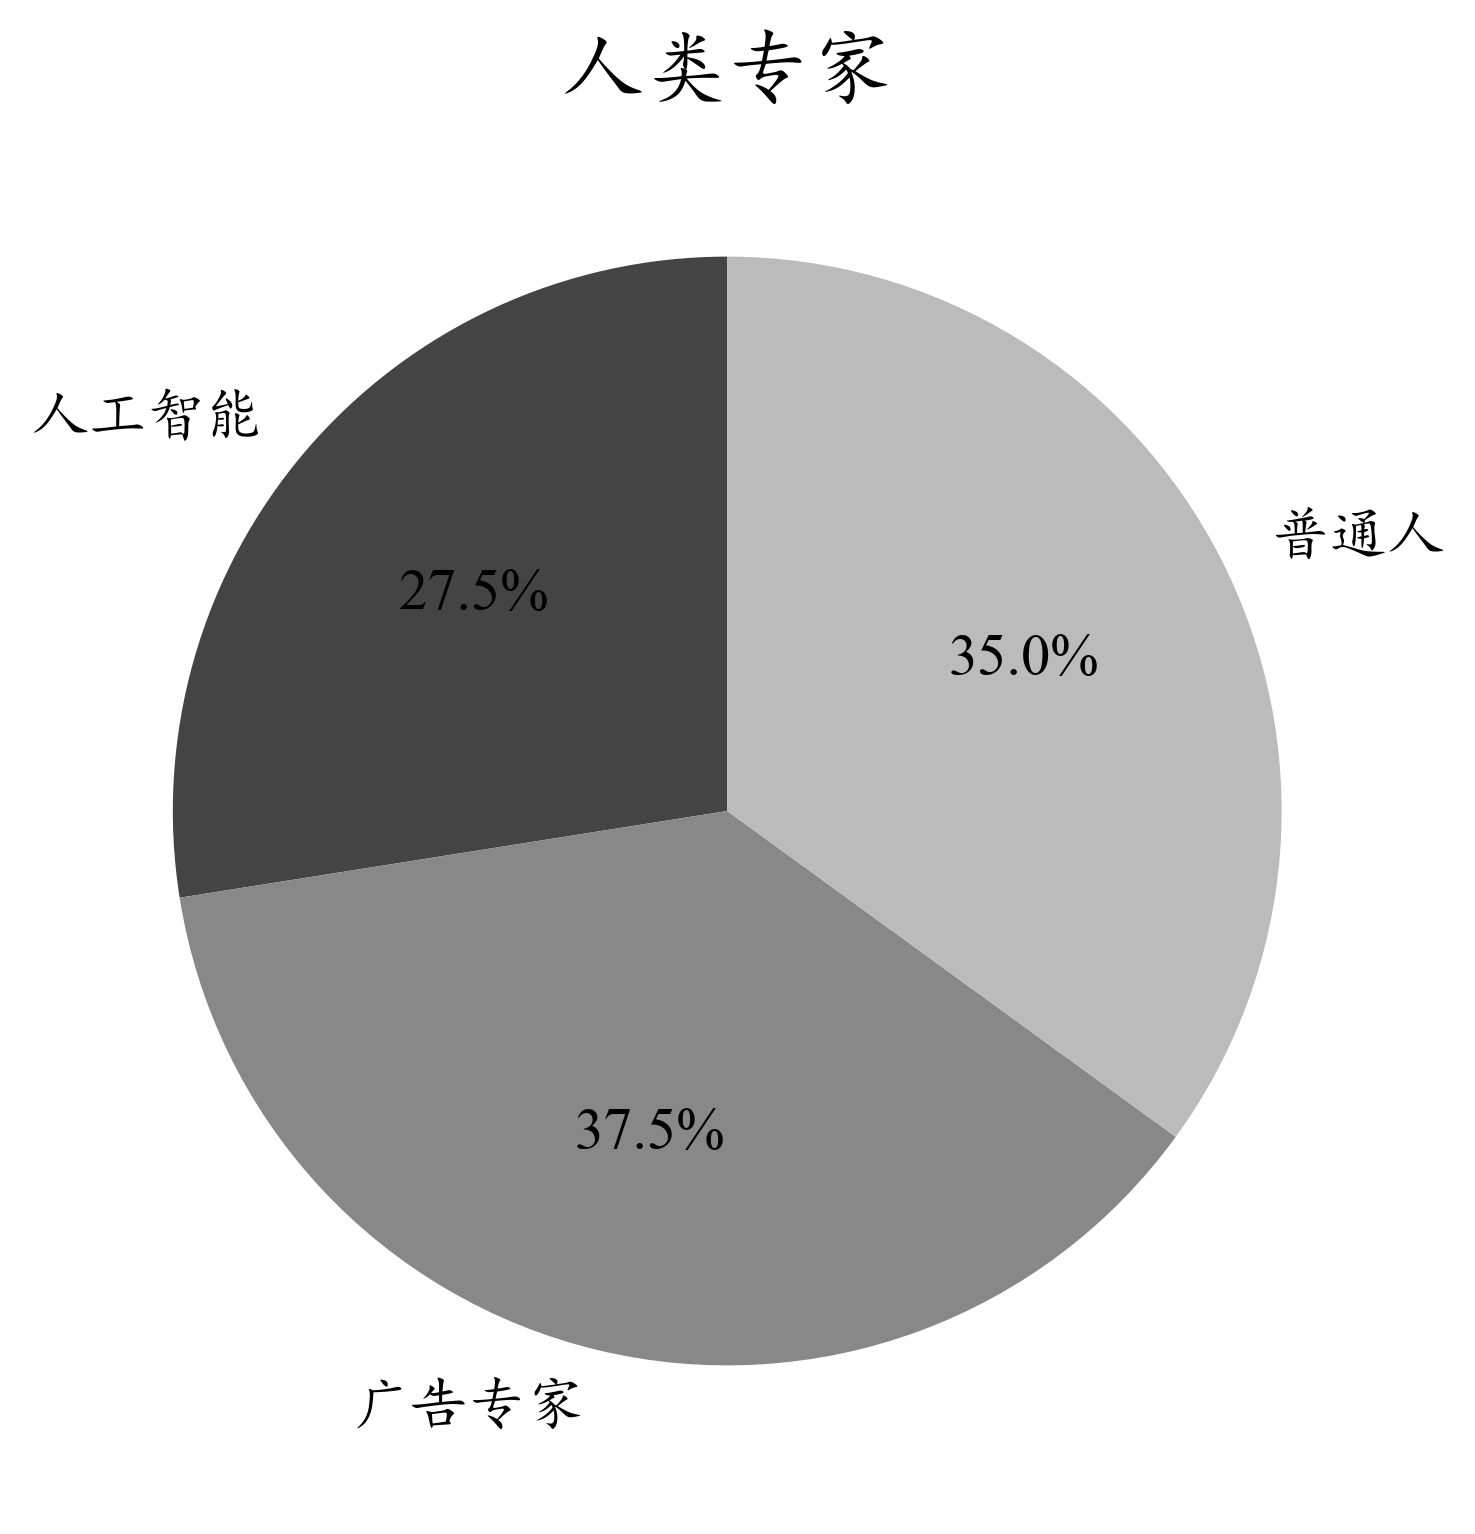
\includegraphics[width=0.4\linewidth]{Image/Study4-exp1-人类专家创作者.png}
    }
    \caption{\label{fig:Study4-exp1-perception} GPT与人类专家实验材料的创作者感知}
\end{figure}

为进一步探讨广告文本的语言特征如何影响受试者对广告来源的推测,本研究基于 LIWC 词法和句法特征进行了单因素方差分析(ANOVA),比较不同广告创作者(AI 生成 vs. 广告专家撰写 vs. 普通人撰写)之间的语言差异。分析结果表明(如表\ref{tab:Study4-substudy1-linguistic_features},不同来源的广告在词汇复杂度、句法结构、指代用法、否定表达、语气表达及冠词使用等方面存在显著差异。

在词汇复杂度方面,AI 生成的广告文本使用了更多的长单词(Sixltr,即包含六个及以上字母的词),其比例最高(0.152),其次是广告专家(0.149),而普通人撰写的广告使用长单词的比例最低(0.033)。这一结果表明,AI 生成的广告语言可能更加正式和专业,而人类撰写的广告更偏向于口语化表达。此外,在句法复杂度方面,AI 生成的广告在句均词数(WPS)上表现出一定优势(22.98),与广告专家(23.31)相近,但均显著高于普通人撰写的广告(22.26)。这表明 AI 生成的广告倾向于使用更长、更复杂的句子,使文本显得更加流畅和结构化,但同时可能降低其口语化程度。

在代词使用方面,AI 生成的广告文本更少使用不定代词(ipron,如“它”“任何”“每个人”),其使用频率最低(1.14),广告专家次之(1.29),而普通人撰写的广告使用最多(1.57)。这一结果可能表明,AI 在生成文本时更注重信息的清晰性,减少了含糊的指代,而人类撰写的广告则更倾向于随意使用不定代词,使文本更具互动感和自然性。此外,在否定表达和比较表达方面,普通人撰写的广告更倾向于使用否定词(negate,如“不会”“没有”),其使用比例最高(1.12),而广告专家使用最少(0.90),AI 生成的广告位于中间(1.21)。相反,AI 生成的广告在比较级(compare,如“更好”“最佳”)的使用频率最高(3.60),其次是广告专家(3.25),而普通人使用最少(3.06)。这一结果表明,AI 生成的广告更倾向于使用比较表达,可能是为了增强广告的说服力,而人类广告撰写者在表达时更直接、更少使用否定表达。

在语气表达方面,AI 生成的广告更倾向于使用推测性语言(discrep,如“应该”“可能”“可以”),其使用比例最高(2.09),普通人次之(1.82),广告专家最低(1.69)。这表明 AI 生成的广告更容易使用可能性或假设性表达,如“你可以实现……”或“这可能会提升你的体验”,而人类广告撰写者更倾向于使用更加确定性的语言,使广告更具信任感。这一结果说明,AI 生成的广告更偏向于正式表达,而人类撰写的广告更倾向于口语化.

最后,在句子结构方面,AI 生成的广告比普通人撰写的广告更频繁地使用前置词(prepend,如“在……之后”“在……之前”),AI 和广告专家的使用比例相同(1.49),均显著高于普通人(1.18)。这表明 AI 生成的广告文本可能更倾向于使用结构更复杂的句式,而人类撰写的广告更偏向简洁直白的表达方式。

综上所述,AI 生成的广告在多个语言维度上表现出与人类撰写广告的显著差异,尤其是在词汇复杂度、句法复杂度、比较表达、推测性语言和句子结构方面更具特点。这些语言特征可能影响受试者对广告来源的判断,使他们更容易将 AI 生成的广告归因于人工智能,而将人类撰写的广告视为人类专家/普通人创作的内容。


\begin{table}[htbp]
    \centering
    \caption{\label{tab:Study4-substudy1-linguistic_features} 语言特征对比}
    {\tablesongti % 整个表格环境应用宋体六号字体
    \renewcommand{\arraystretch}{1.5} % 调整行距
    \begin{tabular}{l c c c c} % 使用 l 让第一列自动调整
        \toprule
        \textbf{语言特征} & \textbf{\( p \) 值}& \textbf{人工智能} & \textbf{广告专家} & \textbf{普通人} \\
        \midrule
        Sixltr & 0.0004 & 0.1523 & 0.1490 & 0.0329 \\
        WPS & 0.0135 & 22.9795 & 23.3107 & 22.2591 \\
        ipron & 0.0079 & 1.1374 & 1.2979 & 1.5702 \\
        negate & 0.0349 & 1.2136 & 0.9048 & 1.1243 \\
        compare & 0.0288 & 3.6045 & 3.2537 & 3.0647 \\
        discrep & 0.0371 & 2.0909 & 1.6954 & 1.8252 \\
        specart & 0.0421 & 2.2395 & 2.2705 & 1.8440 \\
        prepend & 0.0126 & 1.4974 & 1.4973 & 1.1778 \\
        \bottomrule
    \end{tabular}
    }
\end{table}





\section{实验2:AI标签对个性化广告效果的影响}
实验1的结果表明,即使在未明确告知广告来源的情况下,参与者仍能够在一定程度上区分AI生成和人类创作的广告。这表明AI生成广告在语言特征或表达方式上具有独特之处,使其与人类创作的广告有所不同。然而,消费者不仅会根据广告文本的语言特征来推测广告的来源,还可能受到明示信息的影响。当广告明确标注为“AI生成”时,这一信息是否会进一步影响消费者对广告的感知和接受度?换言之,AI 作为广告的生成者,是否会影响个性化广告的说服力?这一问题尚未得到充分探讨。

个性化广告的有效性依赖于心理契合度(psychological fit),即消费者是否认为广告内容与自身需求高度相关。在这一过程中,感知相似性(perceived similarity) 是个性化广告影响消费者态度的核心心理机制 \citep{teeny2021review}。然而,现有研究较少直接测量感知相似性在个性化广告说服过程中的作用,因此本研究首先验证该变量是否确实在个性化广告与消费者态度之间起中介作用。另一方面,人工智能(AI)因缺乏社交属性,往往被认为是心理距离(psychological distance) 更远的主体\citep{kim2020artificial}。心理距离的增加可能导致消费者AI生成广告的感知相似性降低,从而影响个性化广告的说服效果 \citep{ahn2021ai}。换言之,即便AI生成的广告内容符合消费者特征,其个性化效果仍可能因信息来源的影响而受到削弱。基于此,实验2采用两步研究设计,首先验证感知相似性在个性化广告中的关键作用(实验 2a)。实验 2b 在实验 2a 的基础上,进一步引入 AI 标签,以探讨广告来源(AI 生成 vs. 人类创作)是否会影响个性化广告的效果。

\subsection{实验2a:感知相似性的中介探究}
\subsubsection{方法}
(1)被试

实验通过见数平台发布,共 162 名参与者 自愿参加本研究。其中,19 名参与者因未通过注意力检测被剔除,最终保留 143 名有效被试(年龄范围 = 18-48 岁,\textit{M} = 23.83 岁,\textit{SD} = 4.25),其中女性 96 名。每名受试者在完成实验后获得 2 元人民币 作为报酬。

(2)实验材料

本实验采用研究一实验2中的实验材料(\ref{study1-substudy2-methods}),涉及两类产品(薯片与电脑),分别针对尽责性与开放性两个人格特质进行个性化广告设计。对于每种产品-人格特质的组合,实验材料均包含:中性广告(来自社交媒体的原始广告,不包含特定个性化元素);个性化广告(基于该中性广告生成的针对性广告内容,以匹配目标人格特质)。每位参与者需依次观看四组广告(即两种产品 × 两种人格特质),其中每组包含一则中性广告和一则个性化广告。广告呈现顺序随机。观看后,参与者需对每组广告进行评价。

(3)问卷测量

大五人格量表和广告说服效果,测量方法与研究一实验2一致(\ref{study1-substudy2-methods})。除此以外,本实验引入感知相似性 \ref{li2016does},参与者需对以下条目进行评分:“广告的内容符合我的兴趣和需求”,“广告看起来是否像是特地为我设计的”,“广告是否呈现了与我的个性特征相匹配的信息。” 所有测量均采用likert-7点量表(1=完全不同意,7=完全同意),以评估参与者对个性化广告的感知相似程度。

\subsubsection{结果}

在研究一实验2的个性化广告有效的基础上,本实验主要关注感知相似性的中介作用。具体而言,采用 SPSS PROCESS Macro(Model 4) 进行中介效应分析。其中,自变量分别为开放性得分和尽责性得分,因变量为对应个性化广告的说服效果(即开放性个性化广告的效果和尽责性个性化广告的效果),中介变量为感知相似性。

首先,针对开放性维度设计的个性化广告场景(如图\ref{fig:openness-mediation_model}),结果表明开放性得分显著正向预测感知相似性(\textit{b} = 0.8091, \textit{SE} = 0.0892, \textit{t} = 9.0705, \textit{p} < .001),说明高开放性个体更倾向于认为开放性个性化广告符合自身需求。其次,感知相似性显著正向预测广告的说服效果(\textit{b} = 0.5070, \textit{SE} = 0.0335, \textit{t} = 15.1340, \textit{p} < .001)。此外,在控制感知相似性后,开放性得分对广告说服效果的直接效应仍显著(\textit{b} = 0.1289, \textit{SE} = 0.0573, \textit{t} = 2.2482, \textit{p} = .0253)。中介效应分析表明,感知相似性的间接效应为 0.4102,其 95\% 置信区间为 [0.3143, 0.5141],不包含 0,表明感知相似性在开放性个性化广告的个性化效果中起到了中介作用。

\begin{figure}[H] % htbp 让 LaTeX 决定合适的位置
    \centering
    \begin{tikzpicture}[
        node distance=3.5cm,
        every node/.style={align=center, minimum height=1cm, font=\small}, 
        every path/.style={draw, -{Latex[round]}, thick}
    ]
        % 定义变量节点
        \node[draw, rounded corners] (X) {开放性 \\ (自变量)};
        \node[draw, rounded corners, above=of X, xshift=5cm] (M) {感知相似性 \\ (中介变量)};
        \node[draw, rounded corners, right=of X, xshift=5cm] (Y) {个性化说服效果 \\ (因变量)};
        
        % 画箭头,并直接在线上标注路径系数
        \path (X) -- node[midway, above, sloped] {\( 0.8091^{***} \)} (M);
        \path (M) -- node[midway, above, sloped] {\( 0.5070^{***} \)} (Y);
        \path (X) -- node[midway, below, sloped] {\( 0.1289^{*}, 95\% CI=[0.0160, 0.2418] \)} (Y);
        
        % 间接效应标注
        \node[above=0.2cm of M, align=center, font=\small] {
            \textbf{间接效应}: 0.4142, 95\% CI=[0.3143, 0.5141]
        };
        
    \end{tikzpicture}
    \caption{开放性-中介效应模型示意图}
    \label{fig:openness-mediation_model} % 交叉引用时使用 \ref{fig:mediation_model}
\end{figure}

类似地,在针对尽责性维度设计的个性化广告场景中(如图\ref{fig:conscientiousness-mediation_model}),尽责性得分同样显著正向预测感知相似性(\textit{b} = 0.4918, \textit{SE} = 0.0720, \textit{t} = 6.8338, \textit{p} < .001),说明高尽责性个体更倾向于认为尽责性个性化广告符合自身需求。同样,感知相似性显著正向预测广告的说服效果(\textit{b} = 0.4984, \textit{SE} = 0.0298, \textit{t} = 16.7066, \textit{p} < .001)。在控制感知相似性后,尽责性得分对广告说服效果的直接效应仍显著(\textit{b} = 0.1015, \textit{SE} = 0.0392, \textit{t} = 2.5906, \textit{p} = .0101)。中介效应分析表明,感知相似性的间接效应为 0.2451,其 95\% 置信区间为 [0.1566, 0.3388],不包含 0,说明感知相似性在尽责性个性化广告的个性化效果中同样起到了部分中介作用。

\begin{figure}[H] % htbp 让 LaTeX 决定合适的位置
    \centering
    \begin{tikzpicture}[
        node distance=3.5cm,
        every node/.style={align=center, minimum height=1cm, font=\small}, 
        every path/.style={draw, -{Latex[round]}, thick}
    ]
        % 定义变量节点
        \node[draw, rounded corners] (X) {尽责性 \\ (自变量)};
        \node[draw, rounded corners, above=of X, xshift=5cm] (M) {感知相似性 \\ (中介变量)};
        \node[draw, rounded corners, right=of X, xshift=5cm] (Y) {个性化说服效果 \\ (因变量)};
        
        % 画箭头,并直接在线上标注路径系数
        \path (X) -- node[midway, above, sloped] {\( 0.4918^{***} \)} (M);
        \path (M) -- node[midway, above, sloped] {\( 0.4984^{***} \)} (Y);
        \path (X) -- node[midway, below, sloped] {\( 0.1015^{*}, 95\% CI=[0.0244, 0.1785] \)} (Y);
        
        % 间接效应标注
        \node[above=0.2cm of M, align=center, font=\small] {
            \textbf{间接效应}: 0.2351, 95\% CI=[0.1566, 0.3388]
        };
        
    \end{tikzpicture}
    \caption{尽责性-中介效应模型示意图}
    \label{fig:conscientiousness-mediation_model} % 交叉引用时使用 \ref{fig:mediation_model}
\end{figure}


上述分析表明,感知相似性在个性化广告的说服效果中起到了显著的中介作用。即,高开放性/高尽责性的个体在观看与其人格特质匹配的个性化广告时,更倾向于认为广告和自己的相似性,从而增强广告的说服力。此结果验证了感知相似性是个性化广告有效性的关键心理机制,为后续探讨 AI 作为广告生成者是否会影响该机制提供了理论基础。

\subsection{实验2b:AI标签影响的实证研究}
\subsubsection{方法}

本实验采用 $2 \times 2$ 的混合实验设计,其中广告创作者(GPT-4 vs. 人类专家)作为被试间变量,个性化程度(个性化 vs. 非个性化)作为被试内变量。实验旨在探讨 AI 作为广告创作者是否会影响个性化广告的说服效果,并考察个性化广告与信息来源之间的交互作用。


(1)被试

实验通过见数平台发布,共304名参与者自愿参加研究。经注意力检测筛选后,共剔除16名不合格的参与者,最终纳入288名有效被试(年龄范围 = 20-69岁,$\textit{M} = 31.45$,$\textit{SD} = 9.27$),其中146名为女性。所有被试在完成实验后均获得2元人民币作为报酬。

(2)实验材料

本实验选取小米手机(广告中匿名为「M手机」) 在社交媒体上的真实广告文本,并基于该广告文本指导GPT-4生成个性化版本。生成后确保所有广告文本具有相同的产品信息。采用的提示词(prompt)是:“请根据下面的社交媒体上的中性广告内容,修改为两个版本的个性化广告文案,使得目标消费者购买意愿增强,尽管其他消费者不一定喜欢:
1. 针对高外倾性消费者的版本。
2. 针对低外倾性消费者的版本。”

(3)实验流程

在阅读广告材料之前,所有参与者都会根据自己所分配到的条件,被告知特定的广告创造者(cover story)。如果参与者被分配到GPT-4,对广告创作者的描述为:“M手机是一款即将推向市场的智能手机。在本研究中,我们希望了解您对两段广告文案的反馈,以便根据用户反馈优化广告设计。您即将看到的广告文案是由 GPT-4 生成的。GPT-4 是 OpenAI 开发的一款先进的人工智能模型,专门用于理解和生成文本。” 如果参与者被分配到人类专家组,对广告创作者的描述则为:“M 手机是一款即将推向市场的智能手机。在本研究中,我们希望了解您对两段广告文案的反馈,以便根据用户反馈优化广告设计。您即将看到的广告文案是由经验丰富的市场营销专家撰写的,他们擅长创意广告设计和理解消费者心理。” 接下来,所有被试需阅读两则广告文案(一则为针对高外倾设计的广告,一则为低外倾设计的广告),广告呈现顺序随机。参与者需在阅读完每则广告后,完成问卷效果的测量,两则广告评价完后完成人格量表和性别、年龄等人口统计学信息。

(4)问卷测量

a. 说服效果。采用研究一实验2的测量方法(\ref{study1-substudy2-methods})。被试需对广告的说服力进行评分,共包含 5 个题目,采用 1-5 点李克特量表 评分,最终计算平均值作为说服效果得分。

b. 外倾性人格量表:本实验关注外倾性这一人格特质,因此从 \citet{john1991big} 编制的 大五人格量表(BFI-44) 中筛选与外倾性相关的 8 道题目,要求被试根据自身情况进行评分(1=完全不符合,5=完全符合)。

\subsubsection{结果}
首先,为计算个性化水平,本研究以被试的外倾性得分中位数为划分标准,将外倾性得分大于或等于中位数的被试归类为高外倾群体,低于中位数的被试归类为低外倾群体。在广告呈现方面,对于高外倾个体而言,观看专门针对高外倾性设计的广告被定义为个性化广告,而观看针对低外倾性设计的广告则被定义为非个性化广告。相应地,对于低外倾个体而言,观看针对低外倾性设计的广告被定义为个性化广告,而观看针对高外倾性设计的广告则被定义为非个性化广告。

为了探讨广告创作者标签(GPT-4 vs. 人类专家)对个性化广告说服效果的影响,本研究采用了 $2 \times 2$ 的重复测量方差分析,其中个性化(个性化 vs. 非个性化)作为被试内变量,广告创作者标签(GPT-4 vs. 人类专家)作为被试间变量。结果表明(如图\ref{fig:Source_personalization}),个性化与广告创作者标签之间的交互作用达到显著水平,$\textit{F}(1,112) = 6.866, \textit{p} = .010, \eta_p^2 = .058$,表明个性化广告的效果受到广告创作者标签的影响,即标注不同来源的广告在个性化说服力上的表现存在显著差异。进一步的简单效应分析显示,在被标注为人类专家创作的广告中,个性化广告的说服力显著高于非个性化广告(均值差异 = -0.171, 标准误 = 0.092, $\textit{p} = .028$,95\% CI = [0.010, 0.035]),说明当广告被标注为由人类专家撰写时,个性化广告的优势得以体现,受众更容易接受个性化内容。然而,在被标注为 GPT-4 生成的广告中,个性化广告与非个性化广告的说服力差异并不显著(均值差异 = 0.166, 标准误 = 0.090, $\textit{p} = .102$,95\% CI = [-0.023, 0.344]),说明当广告明确标注为 AI 生成时,个性化广告的优势效应被削弱。这一结果表明,即使广告文本内容完全相同,仅仅是信息来源的标注差异,就足以影响个性化广告的说服效果,进一步验证了AI作为信息源在个性化广告中的重要影响。

\begin{figure}[H]
    \centering
    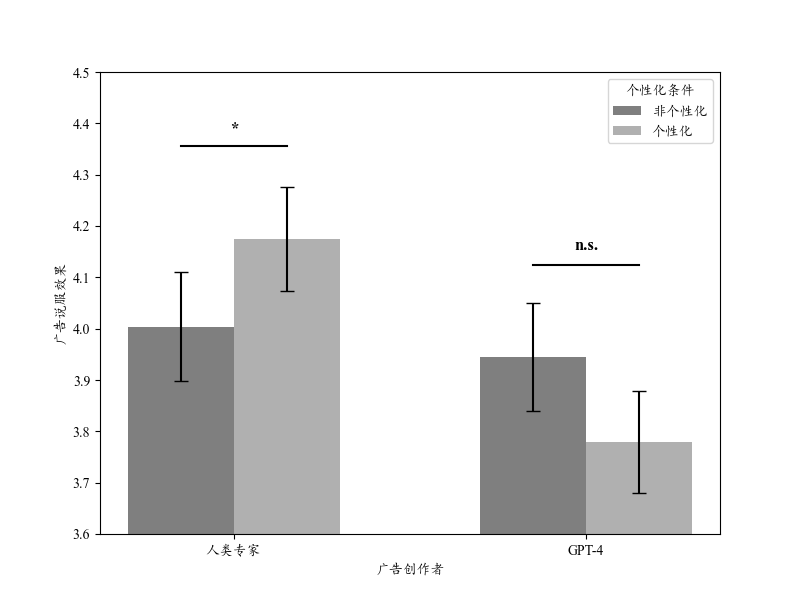
\includegraphics[width=1\linewidth]{Image/Study4-Source_Personalization.png}
    \caption{\label{fig:Source_personalization}广告创作者对个性化广告说服力的影响}
\end{figure}
\section{讨论}

本研究探讨了AI作为个性化广告信息源时对个性化广告效果的影响,并揭示了信息来源在个性化广告的说服过程中所起的关键作用。研究结果表明,个性化广告的有效性受到感知相似性的中介作用,即当受众认为广告内容与自身特质相匹配时,其说服效果更强 \citep{li2016does, teeny2021review}。然而,当 AI 作为广告创作者的身份被明确标注 时,即使广告文本本身符合目标受众的人格特质,其说服力仍然受到削弱。这一发现表明,个性化广告的有效性不仅取决于内容本身,还受到受众对信息来源的认知影响。

在 信息来源认知 方面,研究结果显示,在信息来源未知的情况下,受众能够基于文本特征推测广告创作者,并且 AI 生成的广告在语言风格上与人类专家撰写的广告表现出系统性差异。然而,当信息来源被明确标注为 AI 时,个性化广告的说服力下降,受众对广告的信任度也随之降低。这一现象可以通过 感知相似性在个性化广告中的中介作用 来解释。AI 作为信息源会增加受众与广告之间的心理距离 \citep{kim2020artificial, ahn2021ai},导致受众在认知上将 AI 视为一个较远的主体,从而降低他们与广告的心理契合度,并最终削弱个性化广告的整体效果。

这一发现对 AI 生成个性化广告的优化策略 具有重要启示。首先,AI 生成广告的优化不应仅停留在匹配目标人格特质的语言风格,而应进一步增强广告的“人性化”表达,以提升其交互性和情感共鸣。例如,研究表明,使用第一人称(I/we)和直接面向受众的语言(you)能够增强个性化体验,减少 AI 生成广告与受众之间的心理距离 \citep{markowitz2020communicating}。这种语言策略能够让广告显得更具互动性,使受众更容易产生自我联结,进而提升个性化广告的说服力。

其次,在 AI 生成广告的披露策略 上,应探索 降低 AI 作为信息来源可能带来的负面影响。研究发现,当 AI 生成的内容被描述为“结合专家意见”或“基于大数据精准分析”时,其可信度和接受度会有所提升 \citep{puerta2022human}。因此,在政策可能要求 AI 生成广告必须披露信息来源 的情况下,企业可以调整披露方式,例如 强调 AI 在广告创作中的辅助角色,而非主要创作者,或通过 人机共创(human-in-the-loop)模式 让人类专家优化 AI 生成的广告内容。这一策略不仅可以结合 AI 的 高效性和大规模数据处理能力,还能够 保留人类专家的创造力和情感共鸣能力,使 AI 生成的个性化广告在 提高传播效率的同时,仍然具备较强的个性化吸引力。
